\RequirePackage{plautopatch}
\RequirePackage[l2tabu, orthodox]{nag}

\documentclass[uplatex,dvipdfmx]{jsarticle}
\usepackage{osukalab_pub_doc}
\usepackage{epic,eepic}
\usepackage{graphicx}
\usepackage{amsmath}
\usepackage[all, warning]{onlyamsmath}
\usepackage{siunitx}
\usepackage{txfonts}
\usepackage{amssymb}

\pagestyle{empty}

\headding{浪花研研究会}%修論の場合はこっち
%\headding{卒業論文発表会}%卒論の場合はこっち

\title{重ね合わせを用いた移動ロボットの未知環境走行性能の推定} 

\department{機械工学科}%修論はこっち
%\department{機械工学科目}%卒論はこっち 

\laboratory{フィールドロコモーション研究室}

\author{佐藤　翔亮}

\date{2026年5月22日}%日付確認のこと

\begin{document}

\maketitle
\thispagestyle{empty}


% \section{目次}
% ・目次

% ・緒言

% ・現在の取り組み

% ・今後の取り組み

\section{緒言}
%スケールフリーの走破性評価軸の緒言がこんな感じ
%研究の背景
災害大国である日本では，地震や台風などの自然災害の影響で人間が立ち入ることが極めて困難な環境が多く存在する．このような凹凸の多い不整地や狭隘な環境における探索，調査，復興作業等を人間の代わりに行うために，小型移動ロボットの需要が1995年の阪神淡路大震災以降高まっている．加えて，2011年の東日本大震災および福島第一原発事故以降，有毒ガスや放射線の影響で人間が立ち入ることができない環境でも活動可能な小型移動ロボットの需要が更に高まった．
%こんな移動機構をもつロボットが多くある
このような環境で活動する小型移動ロボットは，複雑な環境での走破性を向上させるために，設計段階から多様なアプローチが考えられてきた．
代表的な例として，複数の移動機構の併用および合体
\cite{Quince,TITANXX,trackwalker,iRobotPackBot}，
新たな移動機構の開発
\cite{DFC,Mecanum_wheel}，
生物に着想を得た移動機構の検証
\cite{asterisk,harvestman_robot,i_centipod_aqua,K3,six_legged_robot}
等が挙げられる．
しかしながら，これらの移動ロボットには，ロボット同士での性能の比較が難しいという課題がある．
その要因の一つとして，移動ロボットの不整地走破性能における一般的な指標が存在しないことが挙げられる．

%先行研究での課題
先行研究における不整地走破性能の評価方法は，段差の高さや斜度，間隙の長さなどのスケールを用いた指標や
\cite{TITANXX,DFC,six_legged_robot,ro-ba}，
ロボットフィールドや実際の災害現場のような特定の環境内における速度や加速度，走破可否といった性能によって検証されてきた
\cite{Quince,trackwalker,i_centipod_aqua}．
%ロボットたちの性能評価の課題点とは
%いままでは，段差やら斜度のスケールや災害現場を再現した特定の環境における走破可否から検証されてる
%でも，スケール感覚が把握しにくくて，実際の現場でどう動くかは未知数だった
このような方法では，人間サイズのロボットが10~cmの段差を乗り越えた場合と，10~cmサイズのロボットが10~cmの段差を乗り越えた場合では，両者の差異を区別できない．
つまり，これらの手法による評価はロボットの大きさに依存するため，大きさの異なるロボット間での性能比較には適していない．
加えて，特定の環境における走破性能しか評価できないため，実際の現場の不整地における走破性能を予測することも困難である．

%そこで，新しい性能評価ができるようになるとおもしろい
そこで本研究では，様々な地形や環境における走行性能をロボットの大きさに依存せずに評価できる手法の構築を目指す．
本手法は，不整地を周波数表現することで移動ロボットのスケールと地形のスケールの関係を捉えるというものである(Fig.~\ref{fig:概要図})．
従来のスケールによる個別の評価や時間領域での評価ではなく，地形を空間的な波として捉え，その周波数成分を変化させた地形の上を走行させたときの移動ロボットの走行性能を，応答特性として評価する．
%sin波で見れば移動ロボットの走行性能を一般化できるのではないかと考えた．
このように，移動ロボットの走破性を周波数領域で評価することで，様々な地形に応じた走行性能を評価できると考えた．

%この手法を使ってなにか面白いことができるか？
%未知環境における走破性を予測するアプローチを考えた
さらに，この手法を用いることで，未知環境における走破性能を予測することも期待できる．
災害現場は未知環境であり，建物の倒壊等の影響で環境が刻々と変化する．このため，観測するまで地形の形状がわからず，事前に移動ロボットの走破性能を予測することはできない．
未知の不整地を十分滑らかで連続した波であるとして，フーリエ変換の考え方を応用してそれぞれの周波数帯のsin波地形に分解できると仮定する．
このとき，前述したsin波形状の地形の上を走らせて周波数の変化と走破性能の関係の考え方から，この分解した各sin波地形における走破性能を個別に調査して重ね合わせることで，未知の不整地における走破性能を予測できる可能性がある
%（未知環境を分解できると仮定し，走破性の重ね合わせで表現する→イメージ図を貼る）
(Fig.~\ref{fig:未知環境における走破性の予測のイメージ図})．

\begin{figure}[tb!]
    \centering
    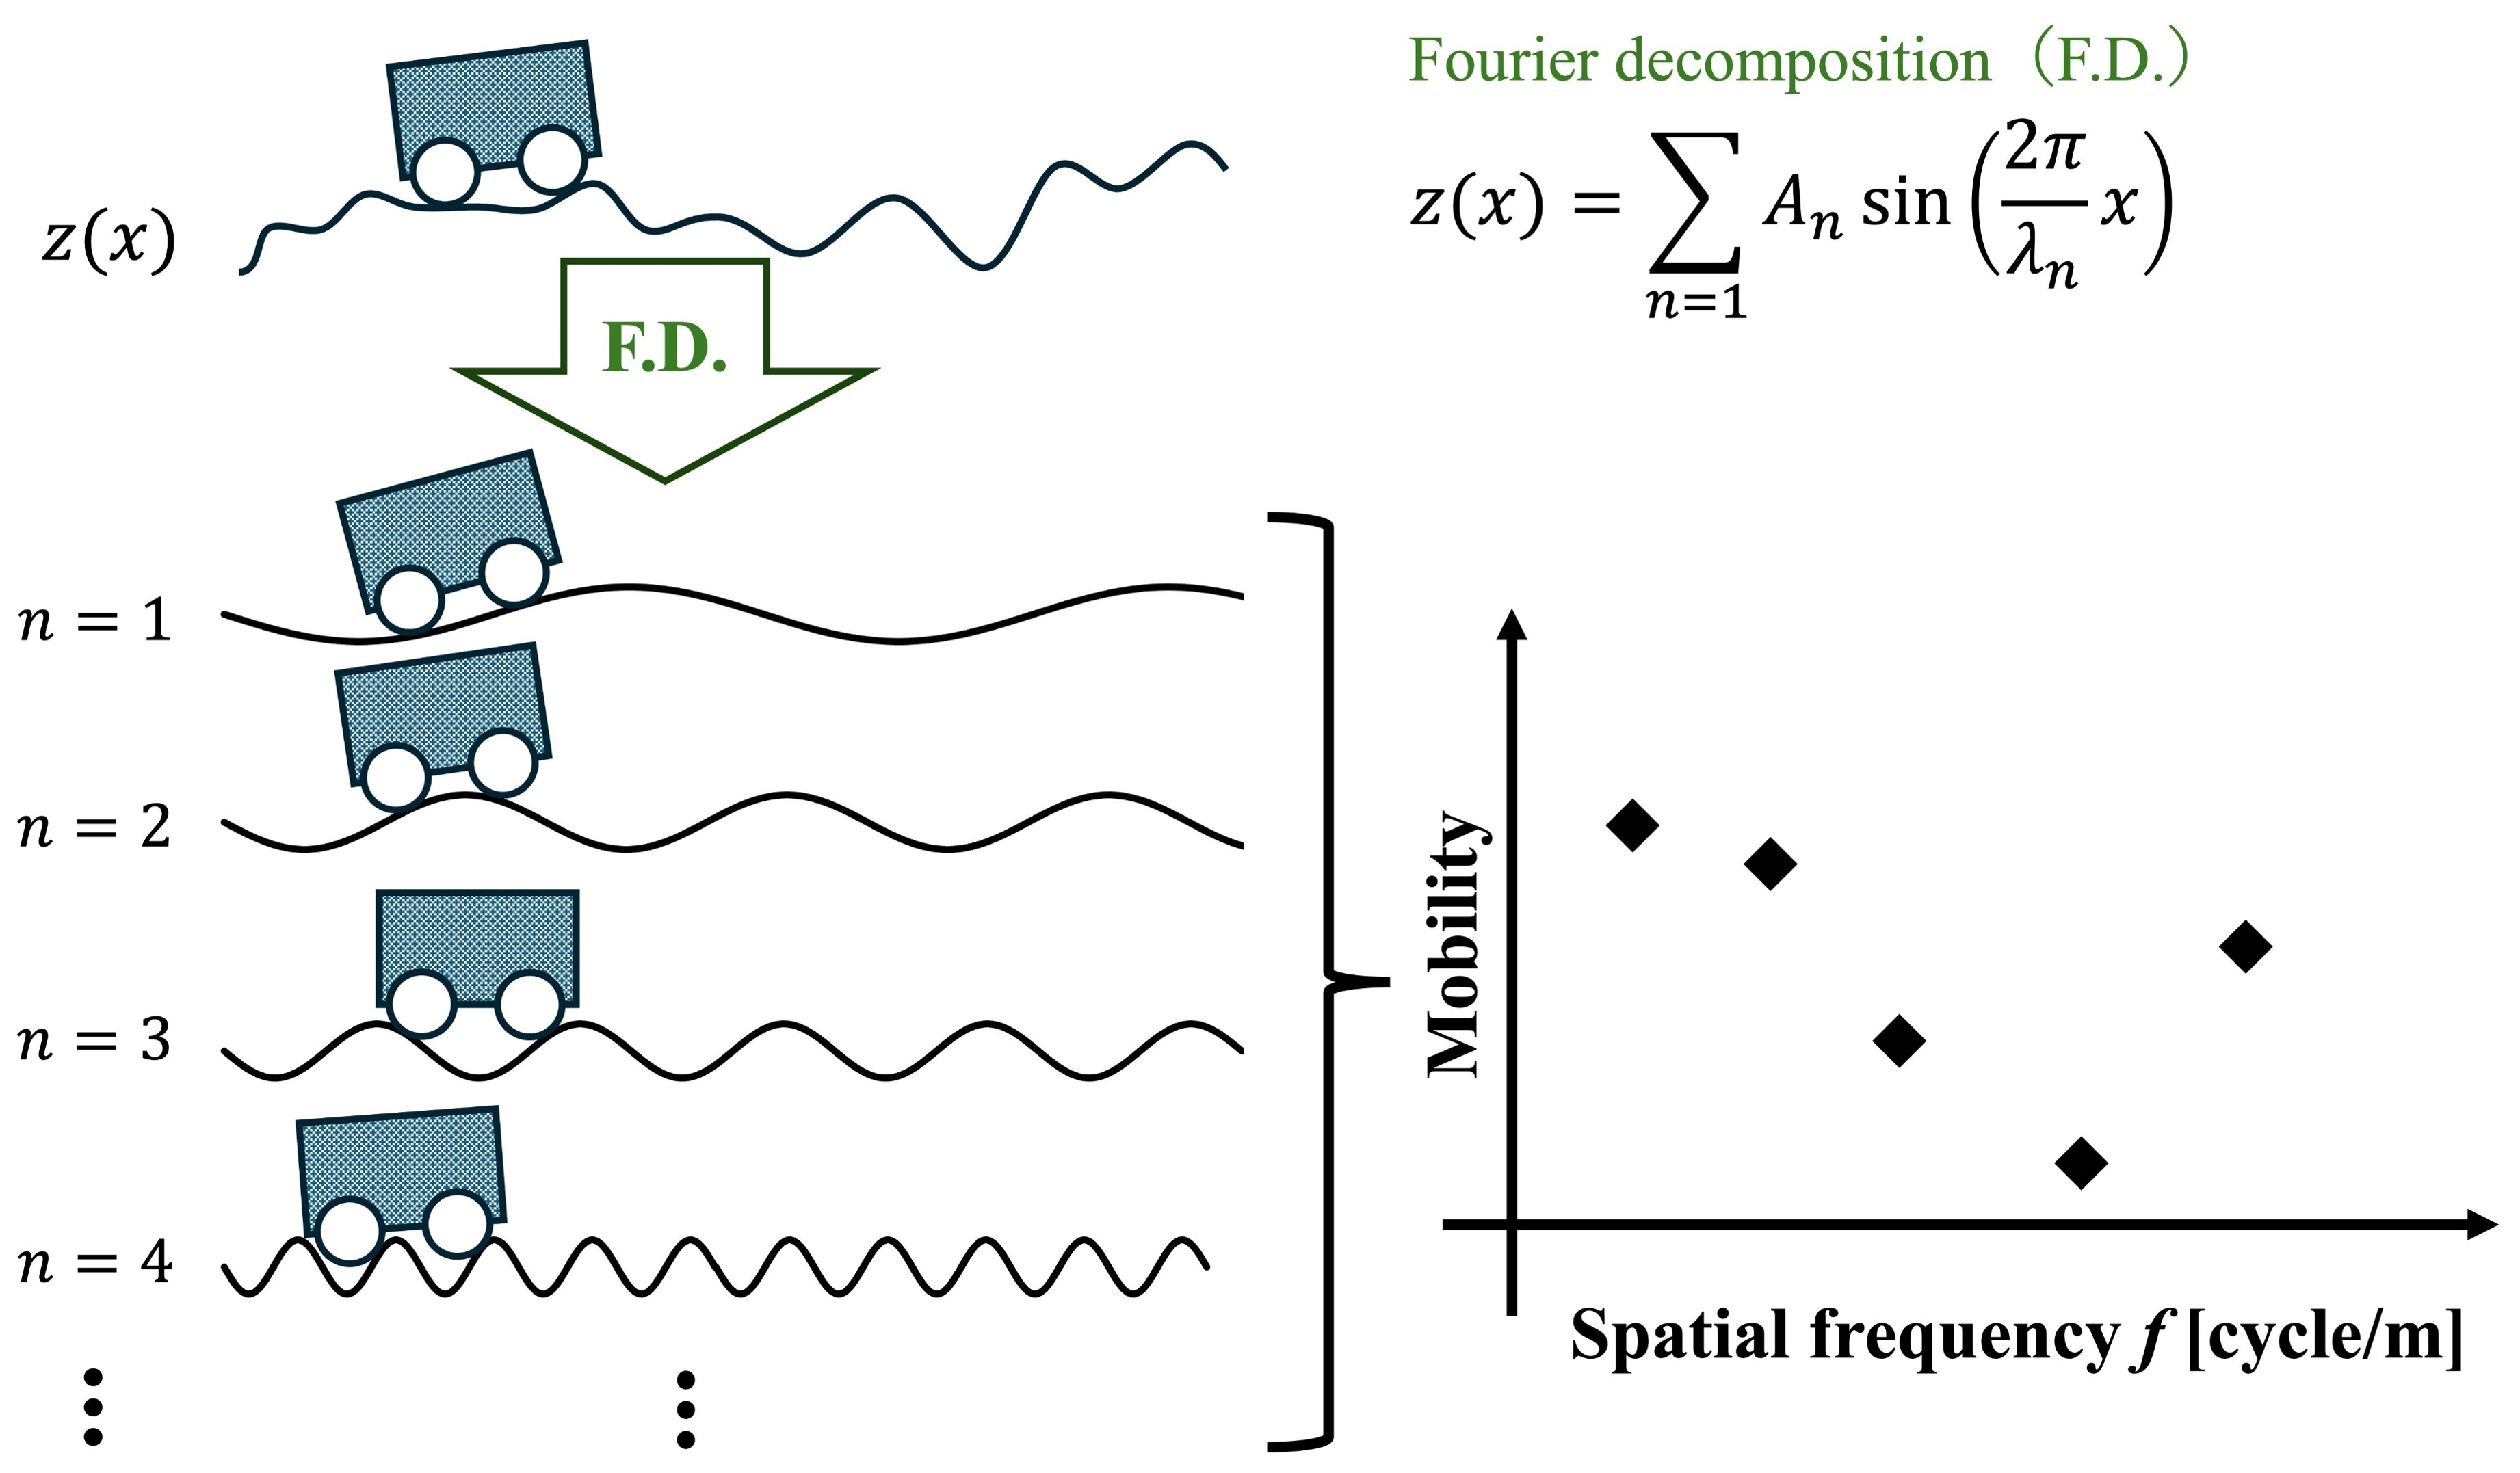
\includegraphics[width=1.0\linewidth]{figure/concept2.jpg}
    %地形周波数表現による走行性能評価の概要図
    \caption{Concept of mobility evaluation using terrain frequency representation}
    \label{fig:概要図}

    \vspace{10pt}

    \centering
    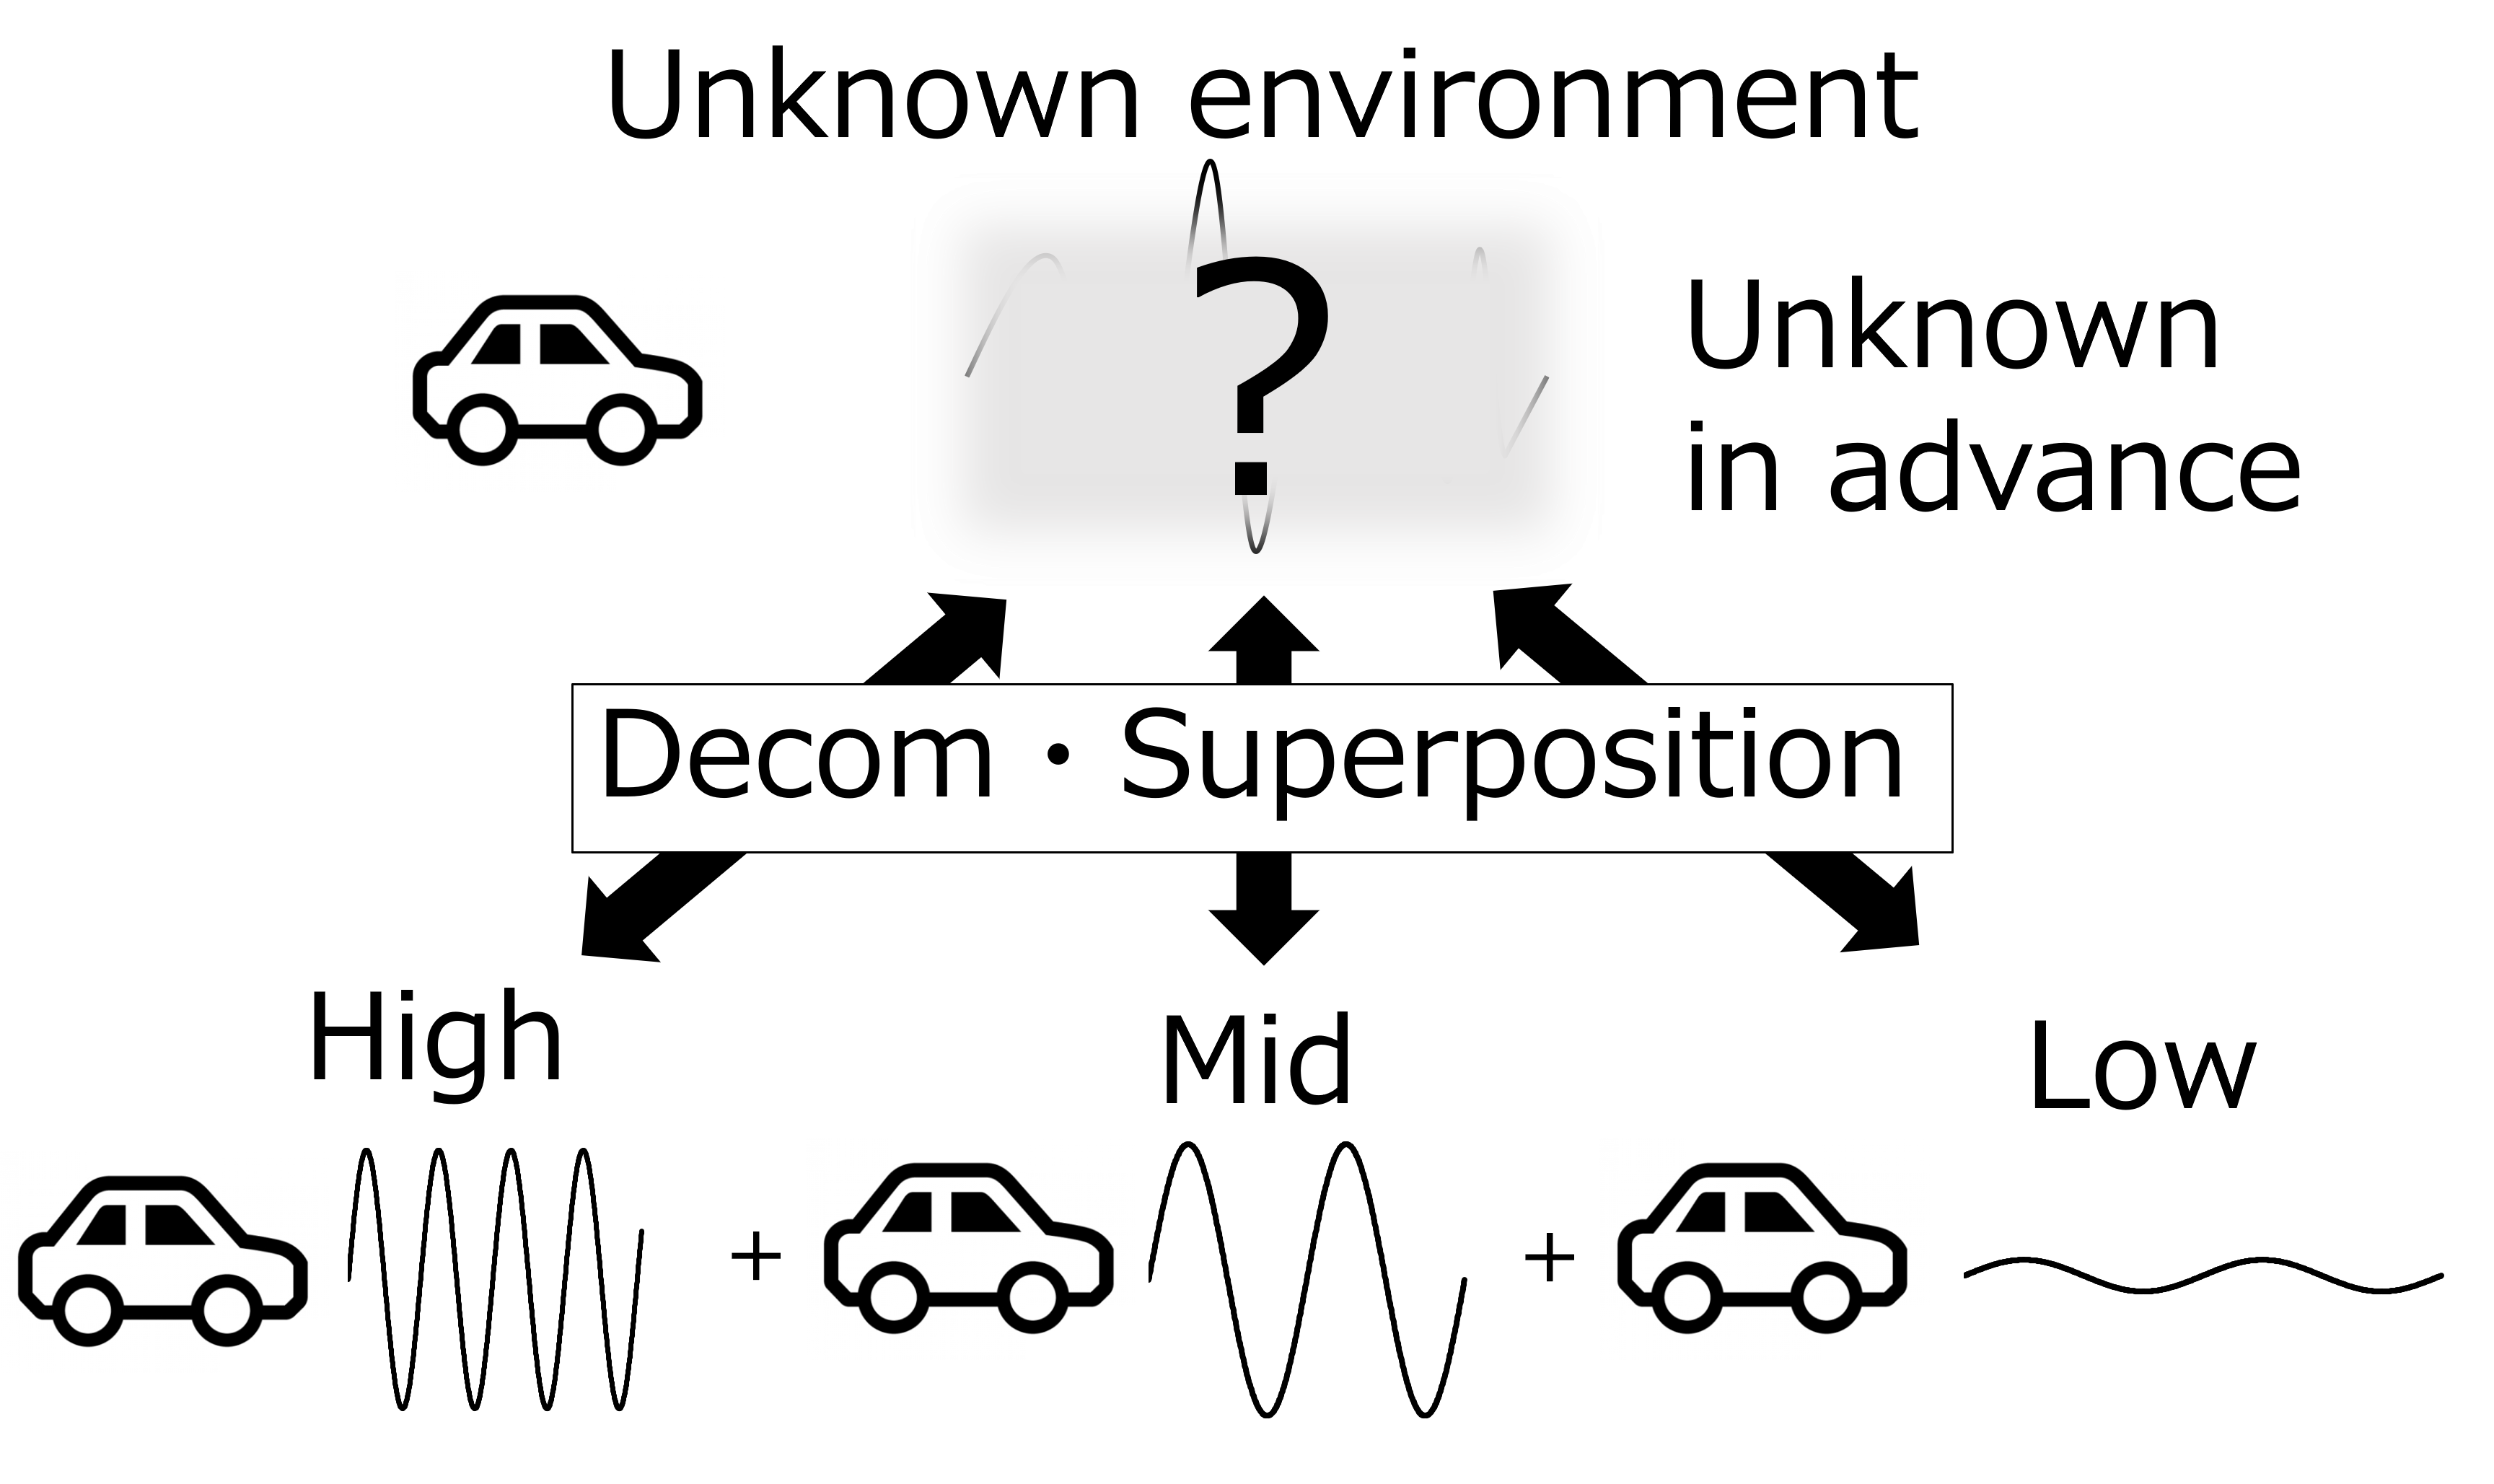
\includegraphics[width=1.0\linewidth]{figure/研究内容のイメージ図.png}
    %未知環境における走破性の予測のイメージ図
    \caption{Concept of mobility evaluation using terrain frequency representation}
    \label{fig:未知環境における走破性の予測のイメージ図}
\end{figure}

%結局なにやるんだ
本研究では，この手法および仮説を検証することを目的とし，本稿では地形を地形を周波数表現することで移動ロボットのスケールと地形のスケールの関係を捉えるという手法について述べる．
本手法では実験に必要な地形のパターンが膨大になることに加えて，移動ロボットのスケールとの関係を調べるために，複数のスケールの移動ロボットを用意する必要がある．
このため，
%実機による評価は困難であると考え，
本手法が走行性能を評価するのに有効かどうかを確認する初期段階として，物理シミュレーションを用いて検証を行った．

% \begin{figure}[tb!]
%     \centering
%     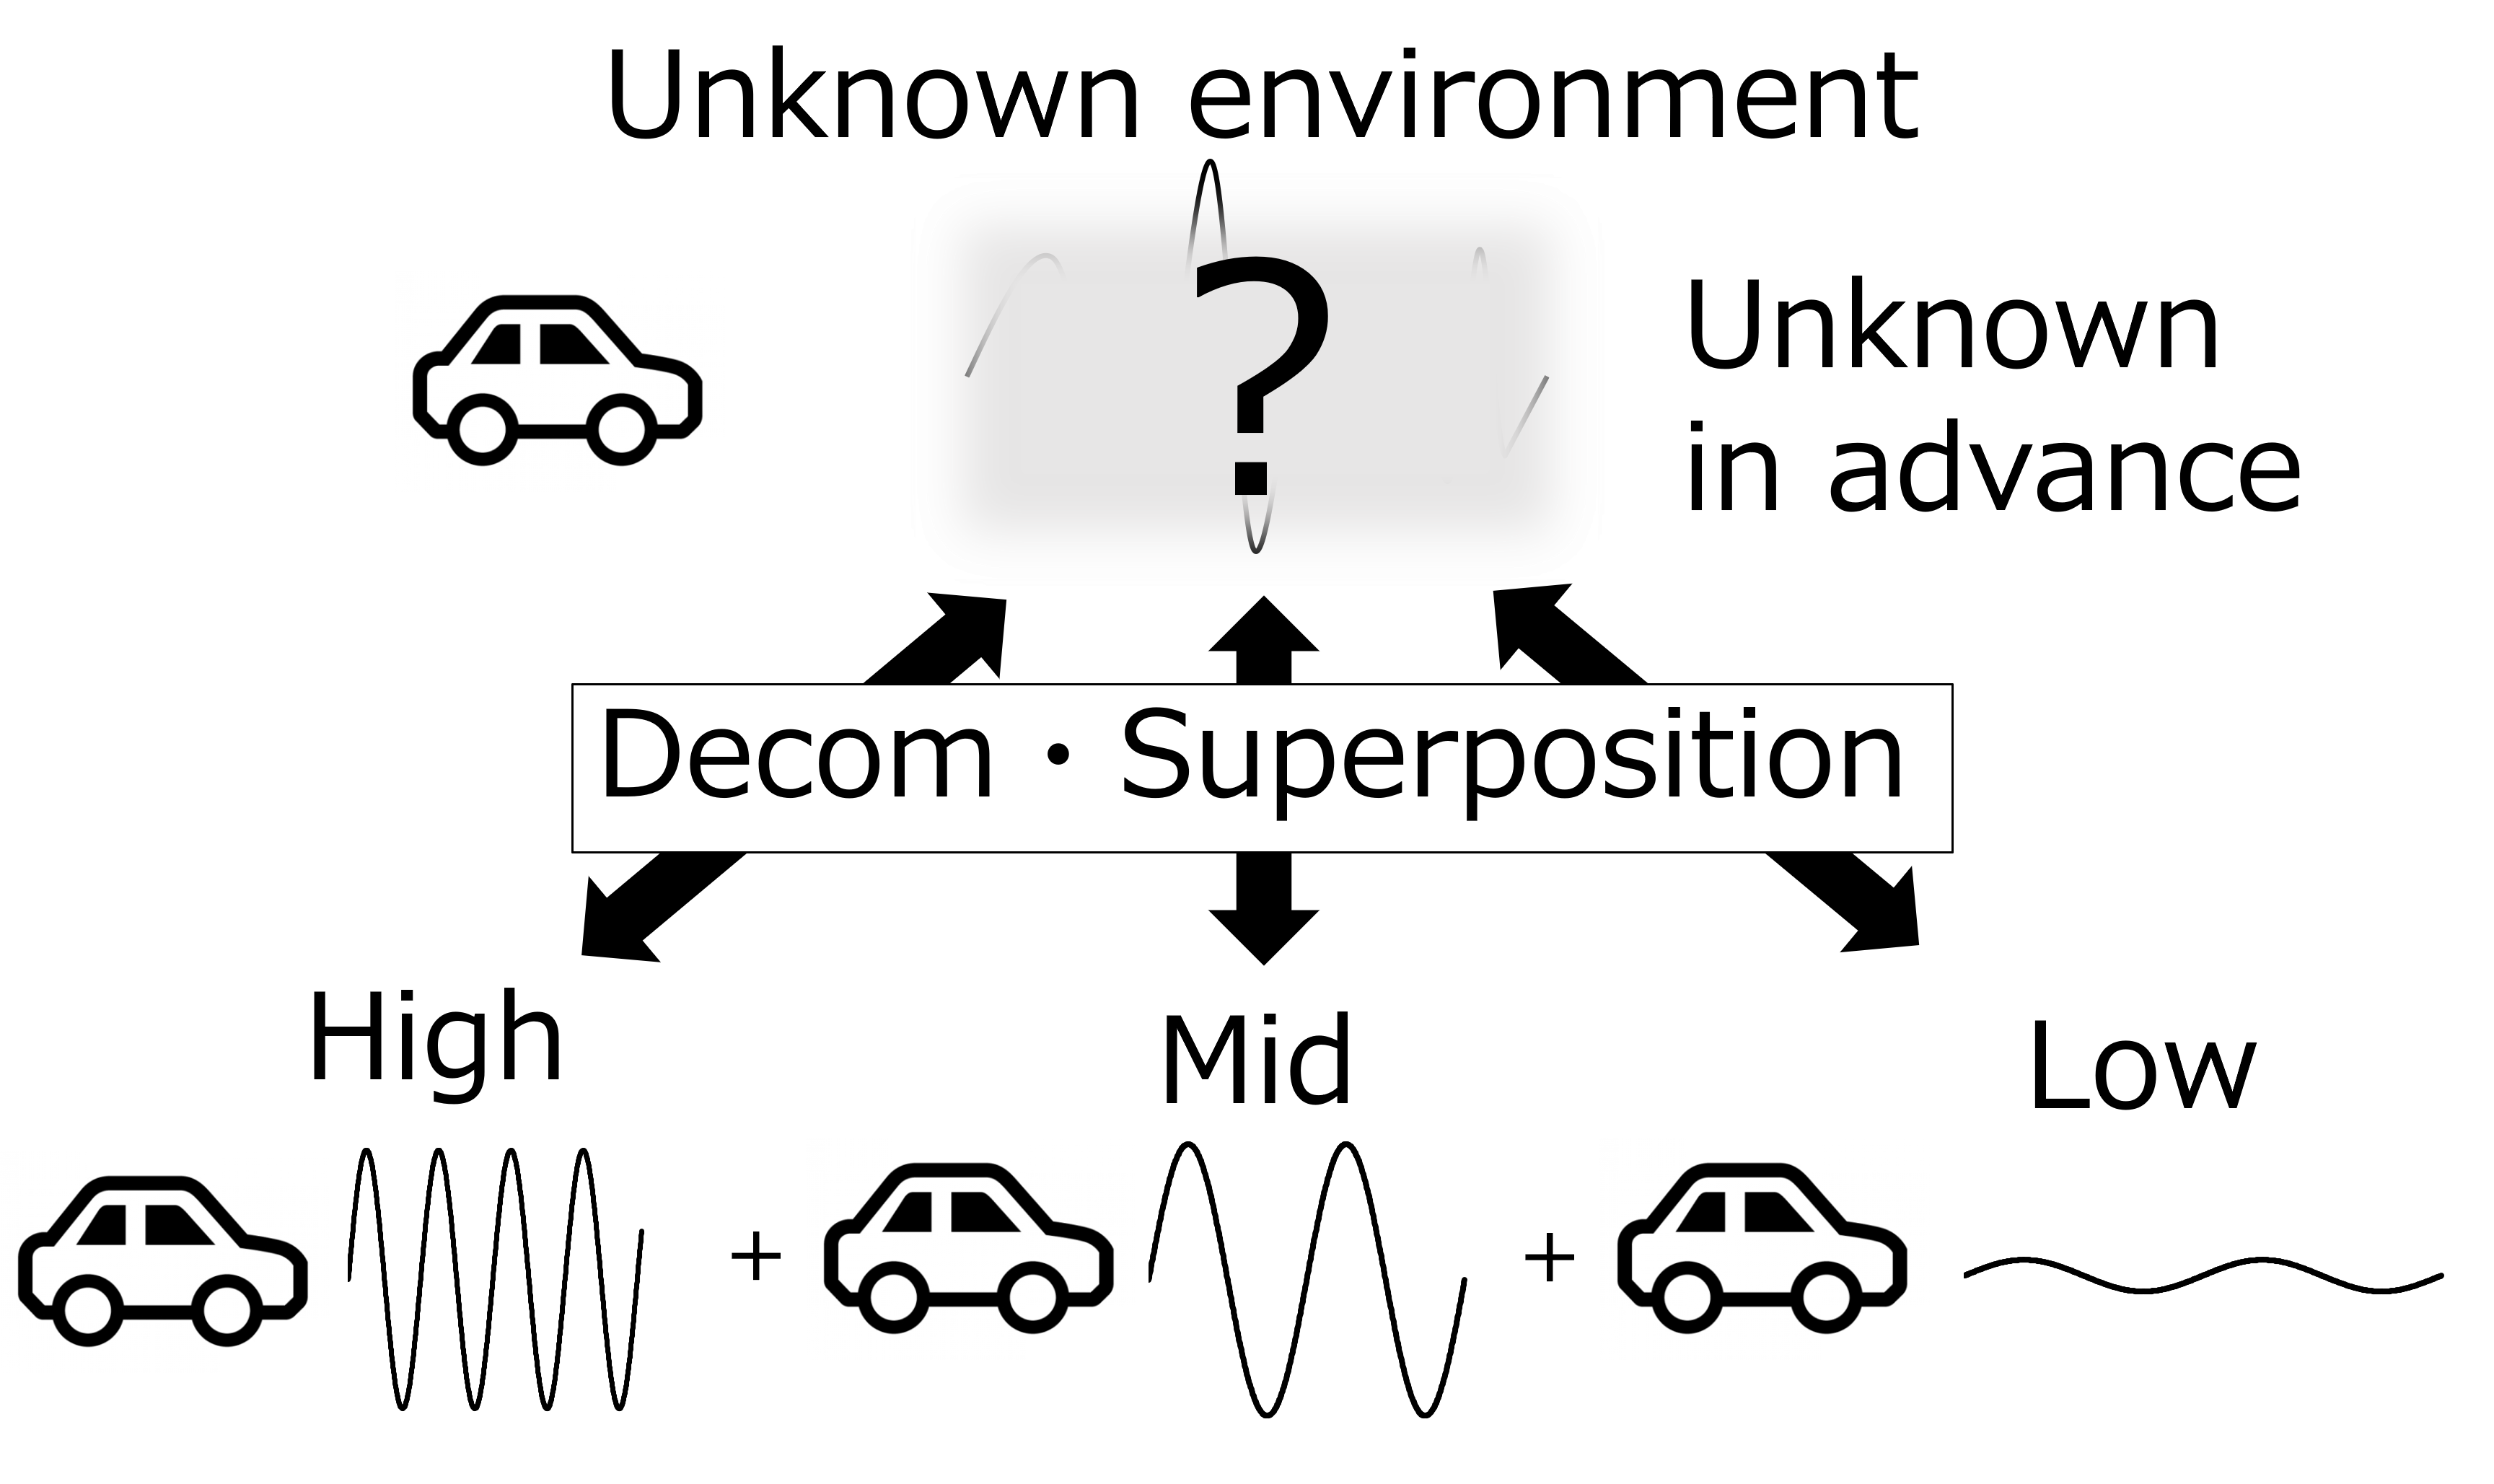
\includegraphics[width=1.0\linewidth]{figure/研究内容のイメージ図.png}
%     %未知環境における走破性の予測のイメージ図
%     \caption{Concept of mobility evaluation using terrain frequency representation}
%     \label{fig:未知環境における走破性の予測のイメージ図}
% \end{figure}

%未知環境軸の緒言がこんなかんじ
%研究背景
%不整地の移動をするロボットの研究が盛ん
%これらの移動ロボットは災害現場等で用いられる
%災害大国である日本では，地震や台風などの自然災害の影響で人間が立ち入ることが極めて困難な環境が多く存在する．このような凹凸の多い不整地や狭隘な環境における探索，調査，復興作業等を人間の代わりに行うために，小型移動ロボットの需要が1995年の阪神淡路大震災以降高まっている．加えて，2011年の東日本大震災および福島第一原発事故以降，有毒ガスや放射線の影響で人間が立ち入ることができない環境でも活動可能な小型移動ロボットの需要が更に高まった．
%でも，災害現場は未知環境と呼ばれ，実際に観測するまでわからない．当然，未知環境における走破性も観測するまでわからない
%現在研究・開発されている移動ロボットは，複雑な環境での走破性を向上させるために，設計段階から多様なアプローチが考えられている．代表的な例として，複数の移動機構の併用および合体（引用），新たな移動機構の開発（引用），生物に着想を得た移動機構の検証（引用）などが挙げられる．

%しかしながら，災害現場は建物の倒壊等の影響で環境が刻々と変化する．このような環境は未知環境と呼ばれ，事前に移動ロボットの走行可否を判断することはできない．
%このため，移動ロボットは機構やらを合体させたり新しい機構を作ってなんとか移動できるようにする，というのが一般的なアプローチになっている．
%そこで，未知環境における走破性を事前に知るためのアプローチとして，不整地をフーリエ変換で分解して，その分解したsin波形状の地形を走らせたときの走破性を，重ね合わせるという手法を提案する．
%そこで，本研究では未知環境における走破性を事前に予測するための仮説を提案する（図を入れる）．
%離散的計算を避けるために連続であると仮定する
%具体的には，未知の不整地を十分滑らかで連続した波であると仮定し，フーリエ変換の考え方を応用してそれぞれの周波数帯のsin波地形に分解する．
%このとき，sin波形状の地形の上を走らせて周波数の変化と走破性の関係を見る．
%この分解した各sin波地形における走破性を個別に調査して重ね合わせることで，未知の不整地における走破性を予測できると考えた．

%この手法における走破性を調べるためには，そもそもsin波形状の地形の上を走らせることで走破性を評価する，という部分について考える必要がある．
%この仮説を検証するためには，sin波形状の地形の上を走らせて，その地形の周波数の変化と走破性の関係を見る
%ことが妥当な評価方法なのかについて考える必要がある．
%という評価方法について考える必要がある．
%具体的な評価イメージは，sin波形状に分解した各地形の上で移動ロボットを走行させ，各sin波地形での平均の速度や身体のがたつき等を記録して一つずつ地形の周波数の変化でプロットしていくというものである．(イメージ張る)

%ここ上と下で話つながらん



%現在の移動ロボットは，異なるロボット同士の性能比較が難しい．なぜなら，一般的な不整地走破性の評価指標が存在しないから．
%現在，各ロボット単体での走破性を確認する，というのが現在主流の走破性評価である．しかし，これでは各ロボット同士で比較が難しい，スケール感も把握しにくい．
%従来，移動ロボットの走破性は段差の高さや斜度，間隙の長さ等のスケールを用いた指標や（引用），ロボットフィールドや実際の不整地のような特定の環境内における速度や加速度，走破可否といった指標によって検証されている（引用）．
%このような方法では，人間サイズのロボットが10 cmの段差を乗り越えた場合と，10 cmサイズのロボットが10 cmの段差を乗り越えた場合では両者の差異を区別できない．
%また，速度や加速度もロボットの大きさに依存している．加えて，特定の環境における走破性しか評価できないため，実際の現場の不整地で走破可能かどうかを予測することは困難である．
%また，一般的な指標も存在しないため，異なるロボット同士の性能比較は簡単にはできない．

%そこで，本研究のsin波による走破性評価を提案する．これにより，段差や間隙の長さをsin波の重ね合わせで表現でき，またsin波とロボットスケールの関係も見やすくなると思われる．


%このような理由から，本研究ではまずsin波地形の周波数の変化と走破性との関係を調べることを目標とする．








\section{提案方式}




\begin{figure*}[t!]
	\centering
	\begin{subfigure}{0.6\textwidth}
		\centering
		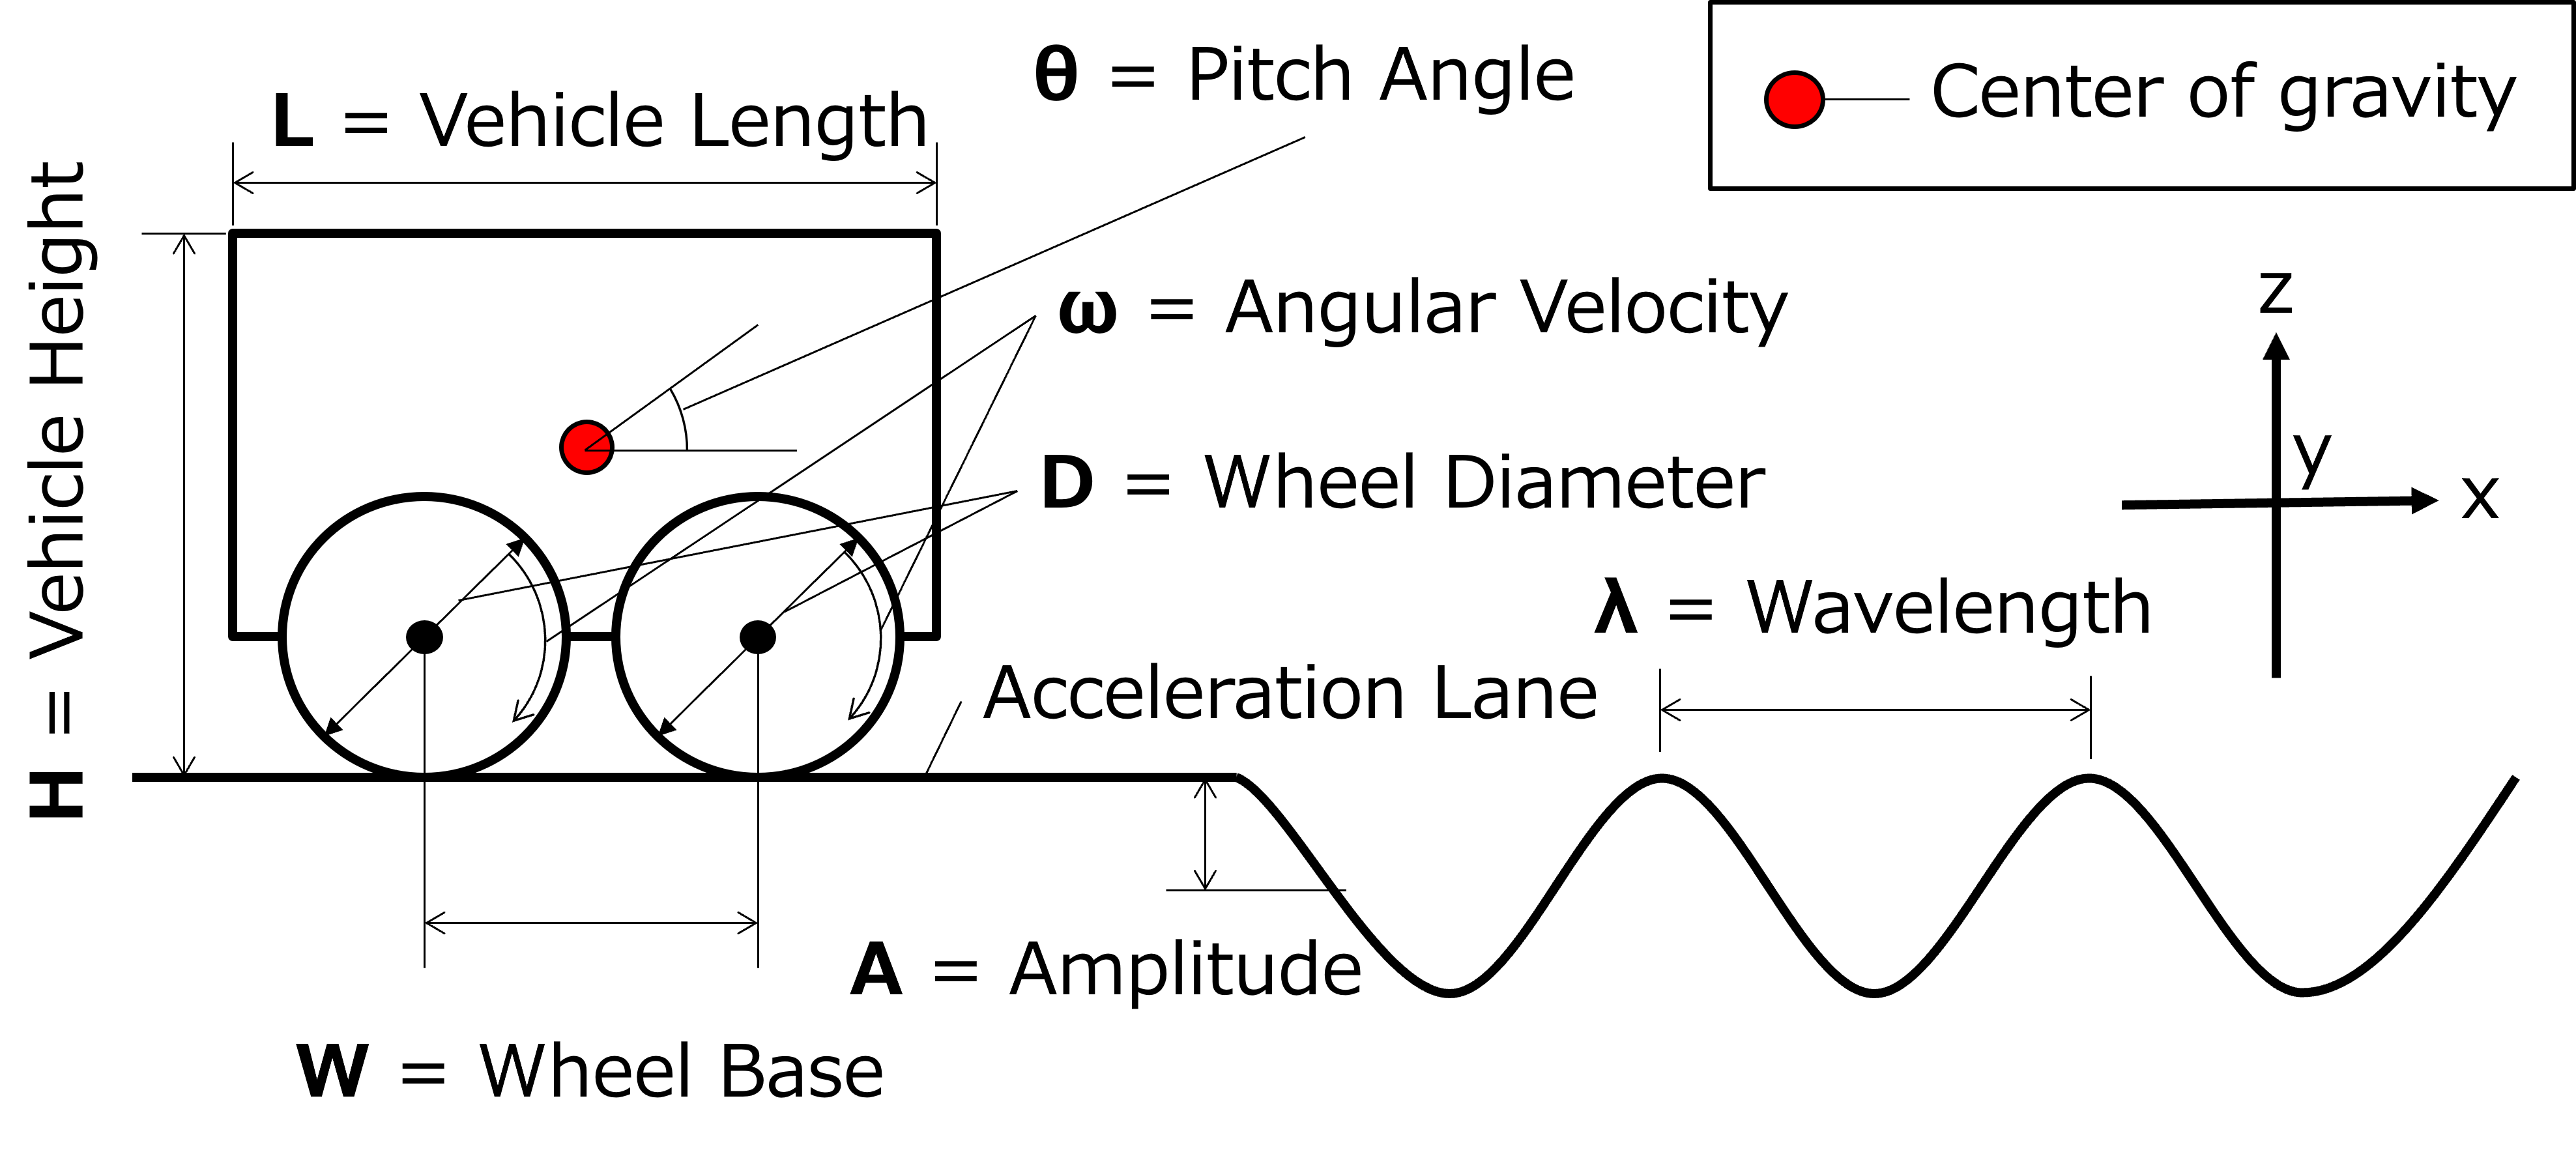
\includegraphics[width=\linewidth]{figure/simimage.png}
		\caption{Simulation of mobility evaluation using frequency characteristics}
		\label{fig:simのイメージ図}
	\end{subfigure}
	\hspace{0.05\textwidth}
	\begin{subfigure}{0.3\textwidth}
		\centering
		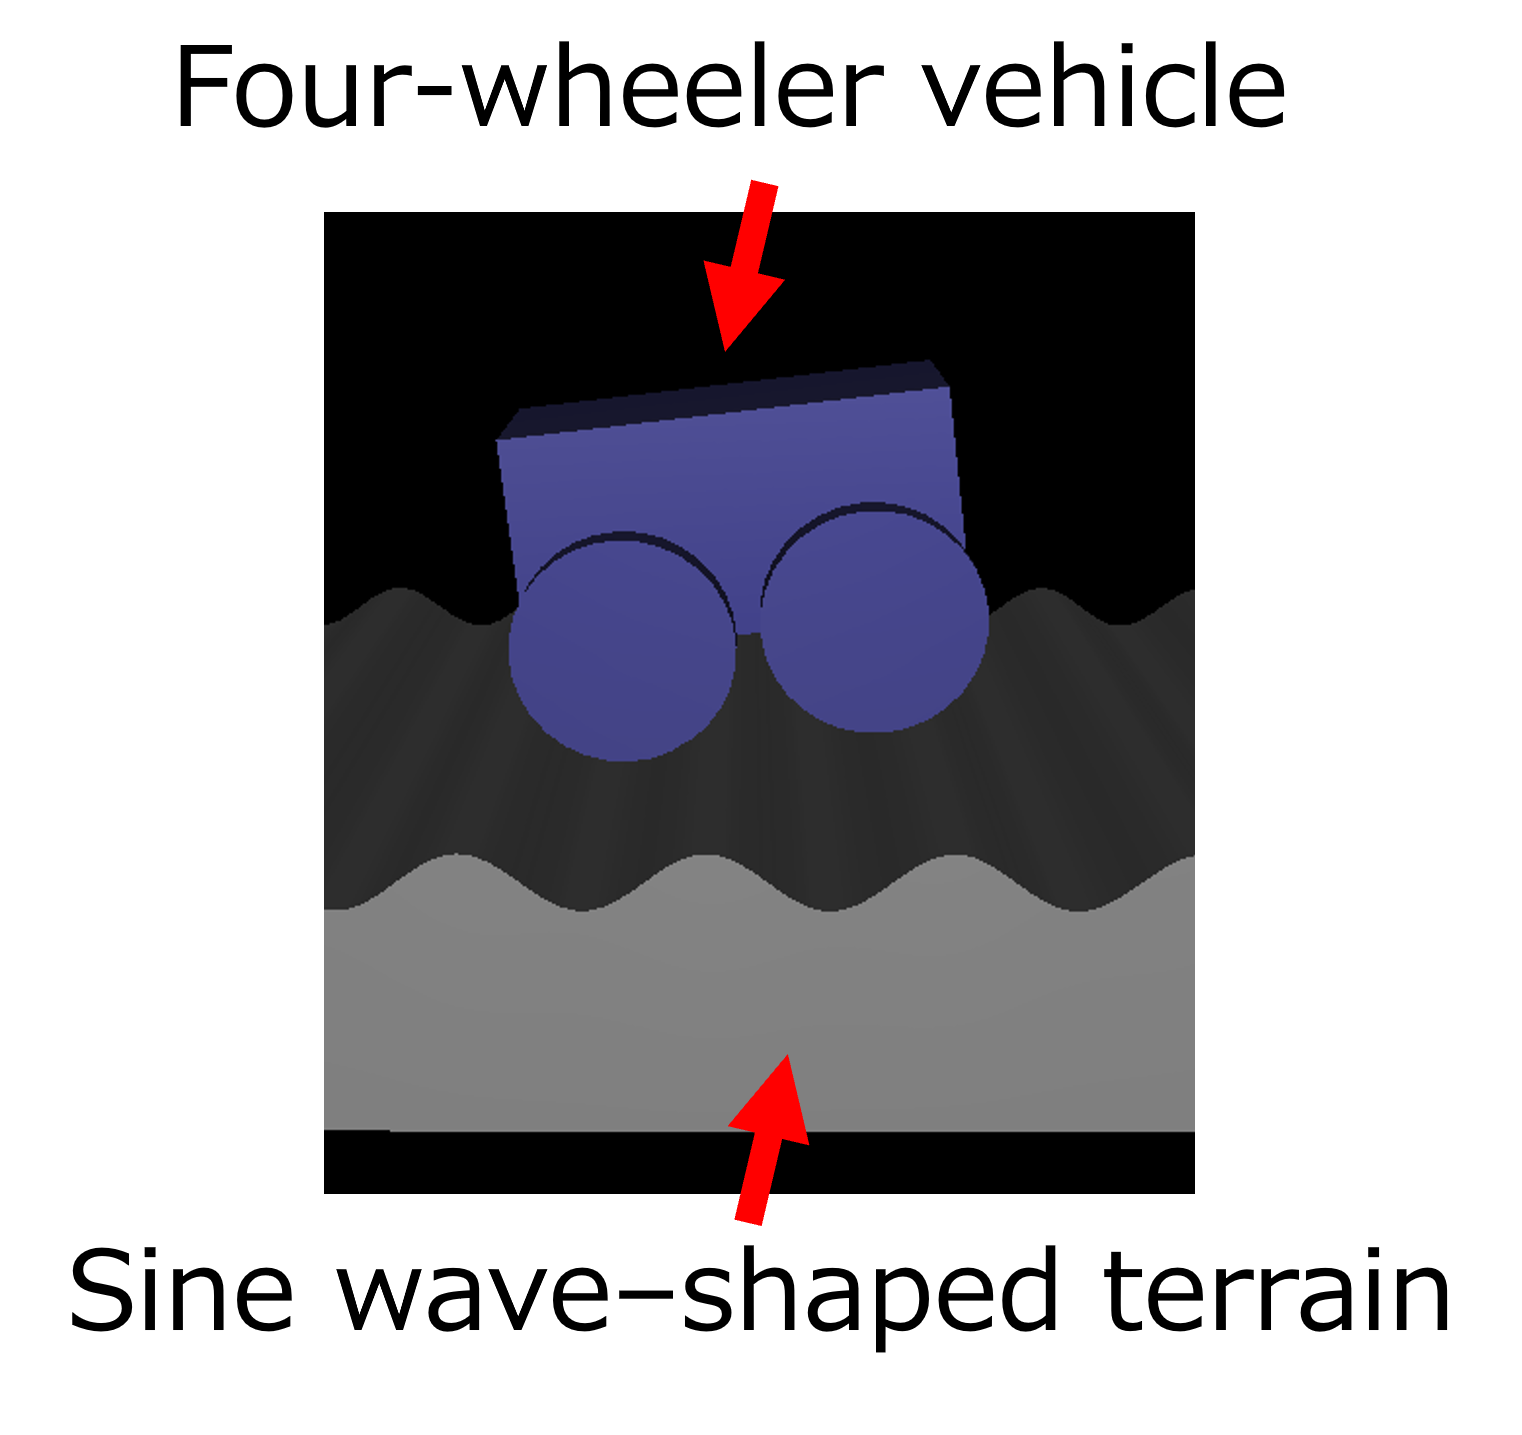
\includegraphics[width=\linewidth]{figure/simshot.png}
		\caption{Screenshot of simulation}
		\label{fig:simスクショ}
	\end{subfigure}
	%シミュレーションの全体構成とスクリーンショット
  \hspace{0.04\textwidth}
	\caption{Overall structure and screenshot of the simulation}
	\label{fig:まとめ図}
\end{figure*}




\section{実験方法}
%\subsection{実験方法}







%\section{現在の取り組み}













% \begin{figure}[tb]
%     \centering
%     \includegraphics[width=1.0
%         \linewidth]{figure/研究概要2.png}
%     \caption{シミュレーションソフトを用いた走行データの取得}
%     \label{fig:研究概要2}
% \end{figure}

  

    % \begin{figure}[tb]
    %     \centering
    %     \includegraphics[width=1.0\linewidth]
    %     {figure/使った車両.jpg}
    %     \caption{シミュレーションに用いる車両 車輪直径60mm 幅150mm 高さ170mm 長さ320mm}
    %     \label{fig:使った車両}
    % \end{figure}

    % \begin{figure}[tb]
    %     \centering
    %     \includegraphics[width=1.0\linewidth]
    %     {figure/四輪車　グラフ.pdf}
    %     \caption{平坦な地形で四輪車を走行させたシミュレーションの変位，速度，加速度のグラフ}
    %     \label{fig:四輪車　グラフ}
    % \end{figure}
   


\section{まとめと今後の展望}






%  参考文献のテスト\cite{bibtest,mike}．

\begin{thebibliography}{99}
  

\bibitem{Quince}
小柳 栄次, サブクローラを持つレスキューロボット, 日本ロボット学会誌, Vol.28, No.2 (2010)  , pp. 147--150

\bibitem{TITANXX}
程島竜一, 福村泰明, 天野久徳, 広瀬茂男, クローラ可変型4足歩行ロボットTITAN Xの開発, 日本ロボット学会誌, Vol.28, No.7 (2010)  , pp. 872--879

\bibitem{trackwalker}
永谷 圭司，秋山 健，吉田 和哉，西田 信一郎, J192011 揺動サイドクローラを有する移動ロボットTrackWalker II による不整地走行実験 : 三原山裹砂漠と中田島砂丘における走行試験, 年次大会, Vol.2012,  (2012)  pp. \_J192011--1--\_J192011--3

%\bibitem{多段クローラ}
%東海林 隆，黒澤 翔，長谷部 順也，藤田 豊己，多段クローラから成る不整地移動ロボットの開発，ロボティクス・メカトロニクス講演会講演論文集，No13-2，Tsukuba，japan，May 22-25 (2016).

\bibitem{iRobotPackBot}
Jessica Gwozdz, N~Morin, Ransom~Philip Mowris, Enabling semi-autonomous manipulation on Irobot’s Packbot, {\em Worcester Polytechnic Institute},  (2014)

\bibitem{DFC}
浪花 啓右，伊東 和輝，佐藤 悠弥，角田 祐輔，衣笠 哲也，谷口 寿俊，三谷 泰浩，大須賀 公一, 双胴柔軟クローラ型ロボット"d-FlexCraw"の走行時姿勢制御と直進性評価, ロボティクスメカトロニクス講演会講演概要集, Vol.2024,  (2024)  pp. 1A1--I05

\bibitem{Mecanum_wheel}
山田 紀之，古村 博隆，遠藤 玄，鈴森 康一, 螺旋形状を持つメカナムホイールによる全方向移動車両の不整地走行実験, ロボティクスメカトロニクス講演会講演概要集, Vol.2016,  (2016)  pp. 2A1--06b3

\bibitem{asterisk}
Tomohito Takubo, Tatsuo Arai, Kenji Inoue, Hikaru Ochi, Takeshi Konishi, Taisuke Tsurutani, Yasuo Hayashibara, Eiji Koyanagi, Integrated Limb Mechanism Robot ASTERISK, {\em Journal of Robotics and Mechatronics}, Vol.18, No.2 (2006)  , pp. 203--214

\bibitem{harvestman_robot}
程島 竜一, ザトウグモの形態を模倣した多脚ロボット, 日本ロボット学会誌, Vol.37, No.2 (2019)  , pp. 138--143

\bibitem{i_centipod_aqua}
山本 誠也，伊東 和輝，角田 祐輔，浪花 啓右，大須賀 公一, 水陸で立ち往生しない多脚ロボットの開発, システム制御情報学会　研究発表講演会講演論文集, Vol.SCI24,  (2024)  pp.~304--308

\bibitem{K3}
浪花 啓右，伊東 和輝，杉本 靖博，角田 祐輔，大須賀 公一, 徹底的に立ち往生しないことを目指した移動機構超多球面脚モジュールロボット：K3（KyuKyaKu）の平面構成走行, システム制御情報学会　研究発表講演会講演論文集, Vol.SCI23,  (2023)  pp.~1D1--06

\bibitem{six_legged_robot}
佐々木 大雅, 藤田 豊己, ６脚クローラ型不整地移動ロボットの開発と溝乗り越え運搬, ロボティクスメカトロニクス講演会講演概要集, Vol.2016,  (2016)  pp. 1P1--06b2

\bibitem{ro-ba}
長塩 拓馬，正岡 宏一，田中 耕治，二次元重心位置制御が可能な車輪型ローバの不整地での走行性能の検討, Proceedings of the 2016 JSME Conference on Robotics and Mechatronics, No.16-2, Yokohama, Japan, June 8-11, 2A2-18a3(1), 2016.

\bibitem{mujoco}
Emanuel Todorov, Tom Erez, Yuval Tassa, MuJoCo: A physics engine for model-based control, {\em 2012 IEEE/RSJ International Conference on Intelligent Robots and Systems}, pp.~5026--5033 (2012)

\end{thebibliography}


{\small
%\bibliographystyle{osukalab}
\bibliographystyle{junsrt}
\bibliography{myref}
\clearpage
\end{document}
}
